\begin{figure*}[t!]
    \centering
    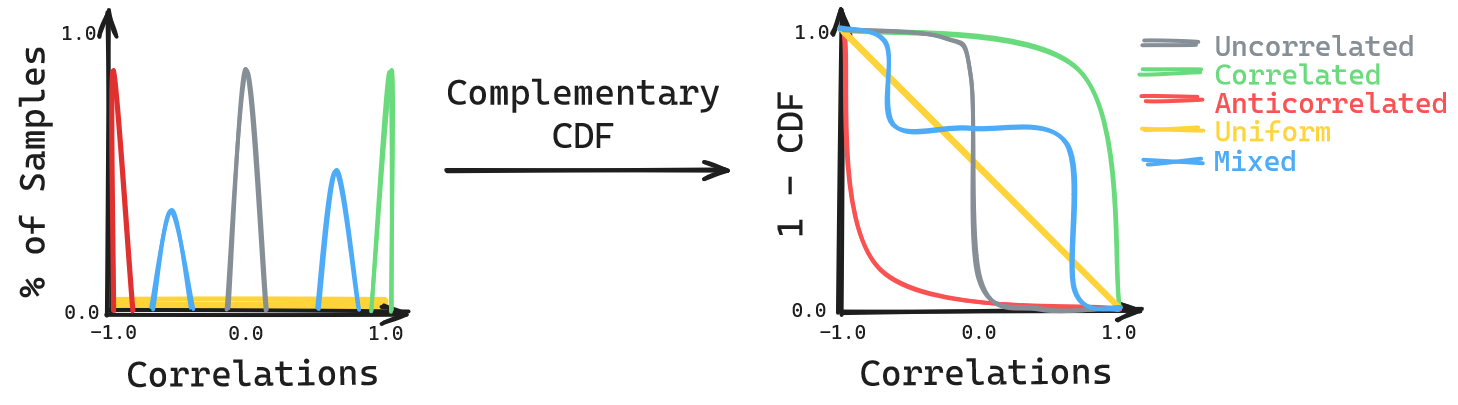
\includegraphics[width=0.9\textwidth]{figures/schematics/Idealized_Survival_Fn6.png}
    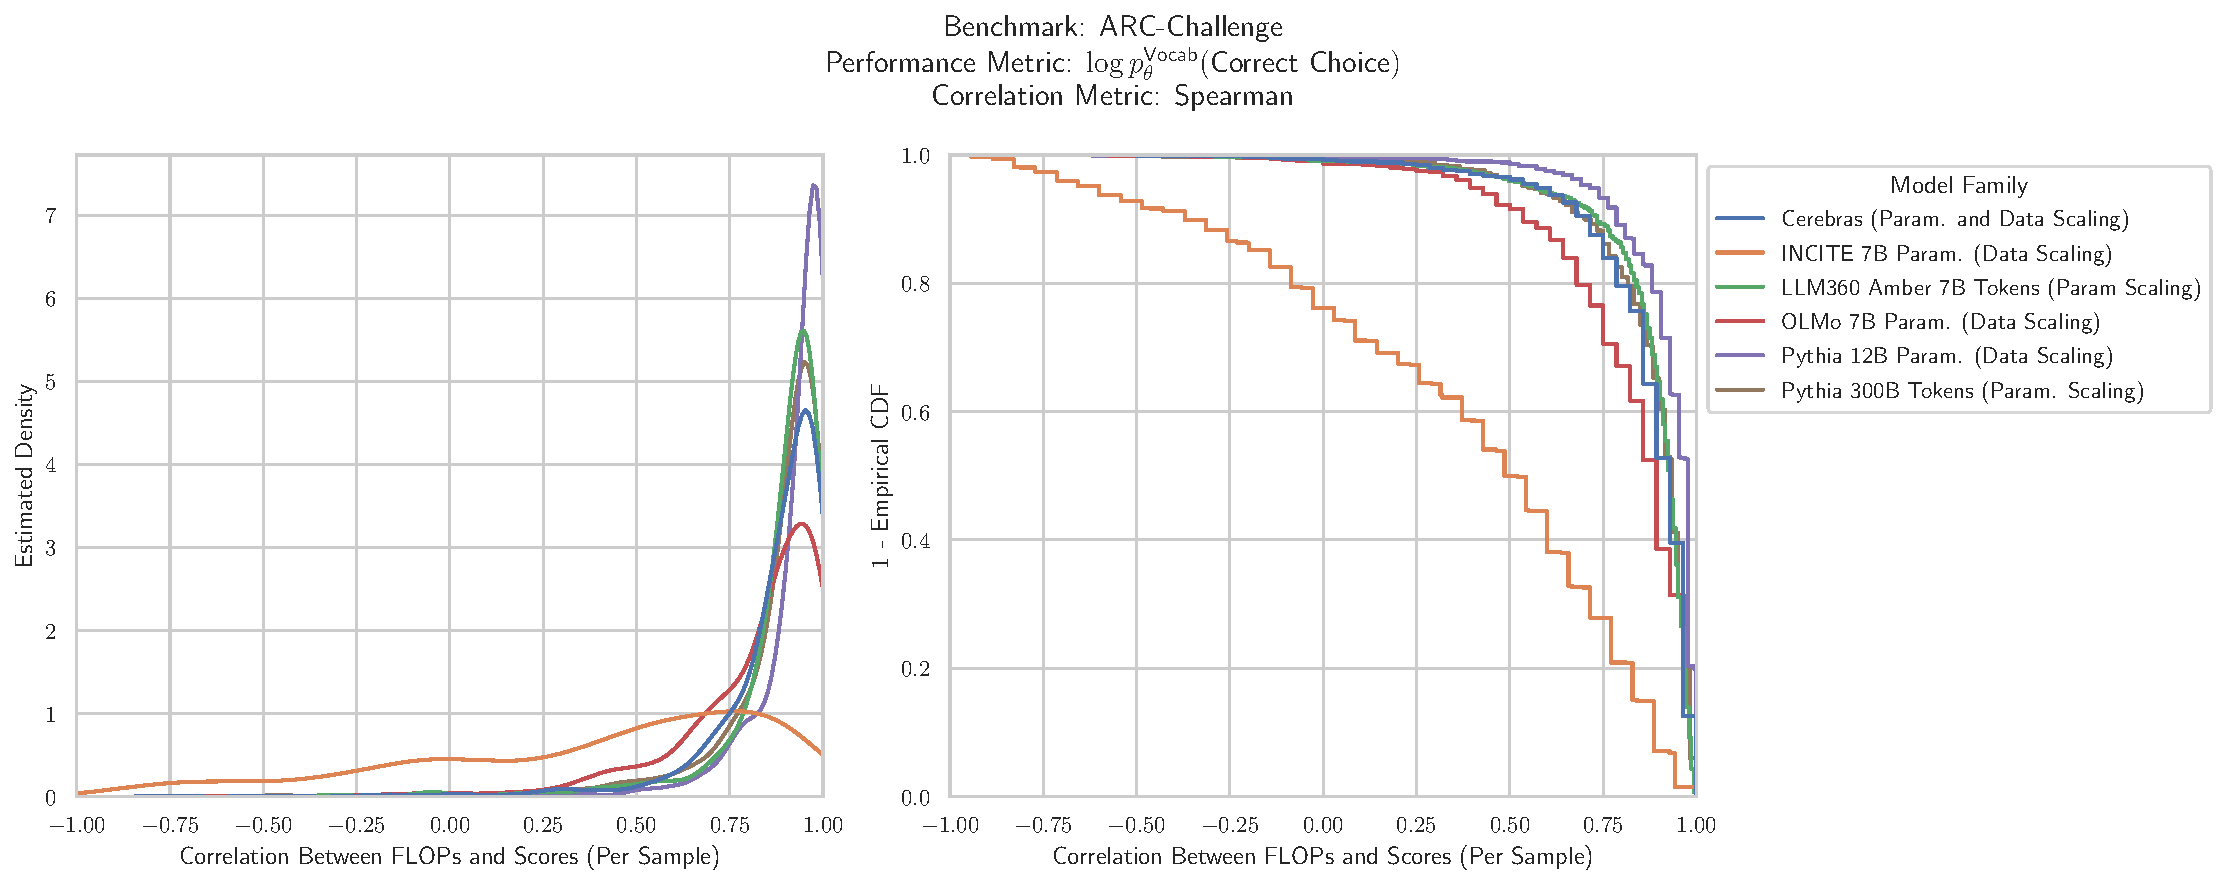
\includegraphics[width=0.9\textwidth]{figures/correlations_between_scores_and_compute/correlation_distributions/arc_challenge/arc_challenge_log_prob_vocab_correct_kde_and_ecdf_vs_correlation_score_by_model_family_correlation_metric=spearman.pdf}
    \caption{\textbf{Distributions of score-compute correlations and their corresponding complementary cumulative distribution functions.} \textbf{Left:} For each benchmark, model family, performance metric, and correlation metric, we computed how scores correlate with compute. This yields a distribution (over samples) of score-compute correlations. Note: the uniform distribution is small but non-zero everywhere. \textbf{Right:} To easily extract what fraction of samples in a benchmark has score-compute correlations above any given threshold, we converted the probability distributions to \textit{complementary cumulative distribution functions}, i.e., $1$ minus the empirical cumulative distribution function (CDF). \textbf{Top:} Idealized distributions. \textbf{Bottom:} Actual data on ARC Challenge.}
    \label{fig:idealized_survival_fn_schematic}
\end{figure*}


\section{What Makes Predicting Downstream Performance Difficult?}\label{sec:what_makes}

Performance on multiple choice benchmarks is commonly published as \texttt{Accuracy}, \texttt{Brier Score}, or probability mass on the correct choice out of the available choices $p_{\theta}^{\text{Choices}}(\text{Correct Choice})$.
These quantities are computed via a sequence of transformations that begins with the negative log likelihood of the correct choice on this particular benchmark sample as some function $f(\cdot, \cdot)$ of compute:
%
\begin{equation*}
    \mathcal{L}_{\theta}^{\text{Vocab}}(\text{Correct Choice}) = f(\text{Compute}, \text{Benchmark Datum})  \label{eqn:loss}
\end{equation*}


\begin{figure*}[t!]
    \centering
    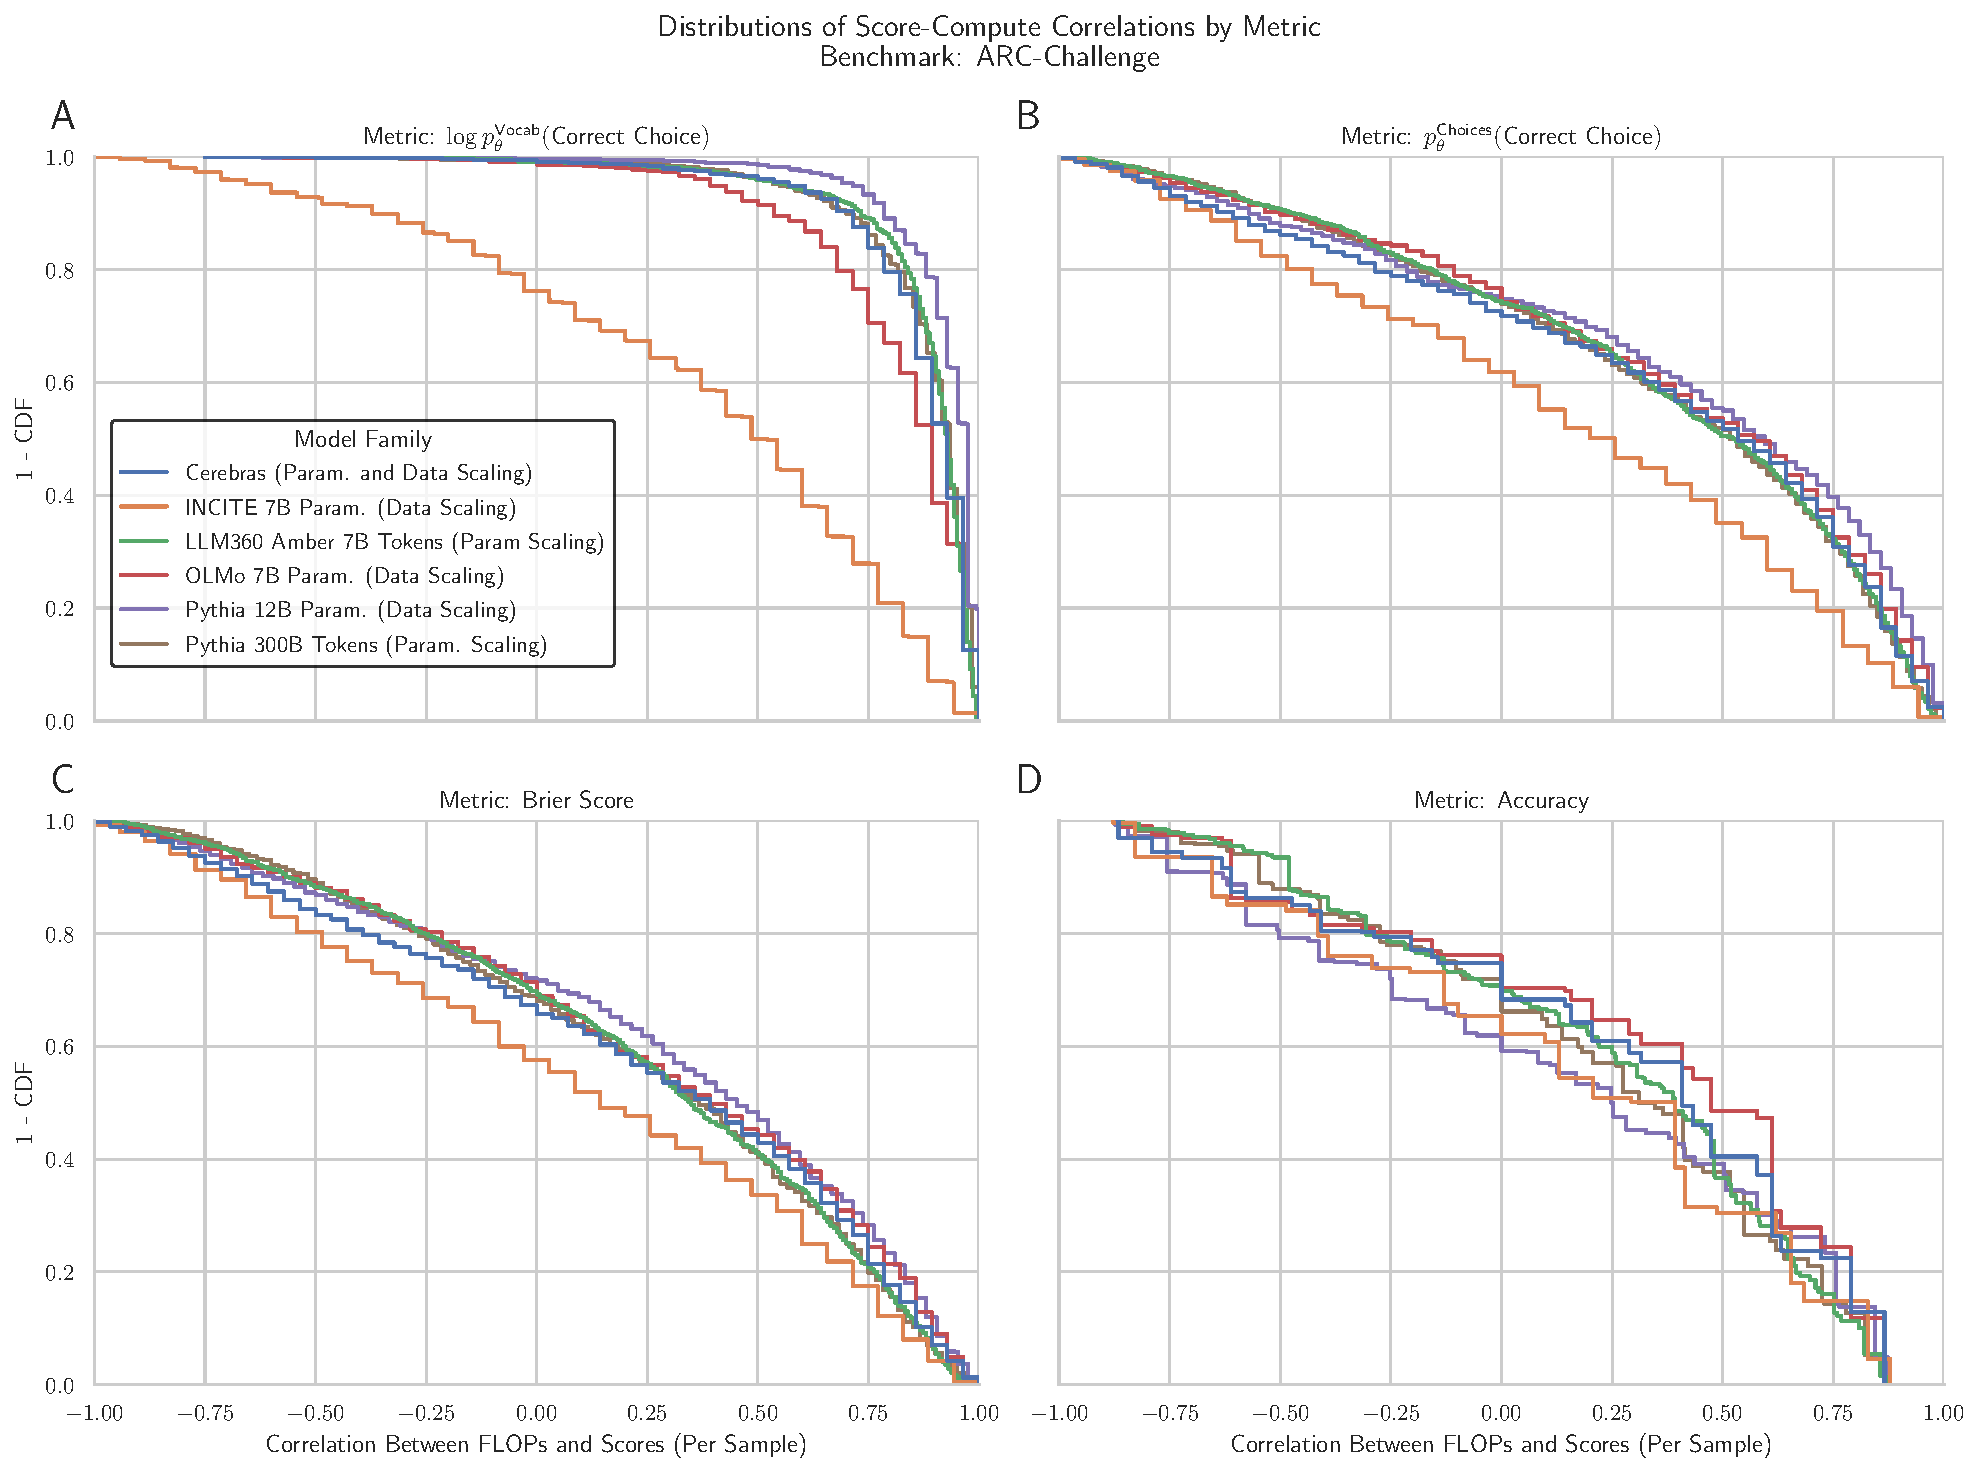
\includegraphics[width=0.9\textwidth]{figures/correlations_between_scores_and_compute/correlation_distributions/arc_challenge/arc_challenge_ecdf_vs_correlation_score_by_model_family_split_performance_metric.pdf}
    \caption{\textbf{Multiple-choice metrics like \texttt{Accuracy} and \texttt{Brier Score} are computed via a sequence of transformations that degrades correlations between performance scores and pretraining compute.} \textbf{(A)} Initially, scores under $\log p_{\theta}^{\text{Vocab}}(\text{Correct Choice})$ and compute are highly correlated. Transforming $\log p_{\theta}^{\text{Vocab}}(\text{Correct Choice}) \rightarrow p_{\theta}^{\text{Vocab}}(\text{Correct Choice})$ has no effect for rank correlations. \textbf{(B)} Transforming $p_{\theta}^{\text{Vocab}}(\text{Correct Choice}) \rightarrow p_{\theta}^{\text{Choices}}(\text{Correct Choice})$ decorrelates scores from compute. \textbf{(C)} Transforming $p_{\theta}^{\text{Choices}}(\text{Correct Choice}) \rightarrow$ \texttt{Brier Score} minorly decreases score-compute correlations. \textbf{(D)} Transforming $p_{\theta}^{\text{Choices}}(\text{Correct Choice})\rightarrow$ \texttt{Accuracy} more substantially decorrelates scores from compute. Correlation: Spearman. Results are consistent across benchmarks and all three correlation metrics (App. \ref{app:sec:additional_score_compute_correlation_distributions}).
    }
    \label{fig:compute_score_distribution_arc_challenge}
\end{figure*}


% \SK{Overall comment: There is some mixing between what is measured at the sample level and what is measured at the population level, e.g., the above equation should have an expectation on the LHS. I suggest working to clarify this.}
Two details are critical. Firstly, this negative log likelihood is not computed in expectation over a corpus; it is specific to this particular singular datum in the benchmark. \textit{All the scores we discuss are per-datum.} Secondly, this negative log likelihood is computed over the vocabulary of the model. One can then compute the probability mass of the correct choice, again with respect to the vocabulary:
%
\begin{equation*}
    p_{\theta}^{\text{Vocab}}(\text{Correct Choice}) = \exp \big(-\mathcal{L}_{\theta}^{\text{Vocab}}(\text{Correct Choice}) \big) \label{eqn:p_correct_vocab}
\end{equation*}
%
% \SK{prior notation is unclear, perhaps consider verbose as $\{ \text{Available Choice}_{1}, \text{Available Choice}_{2}, \ldots, \text{Available Choice}_{K} \}$ Perhaps do verbose once to define notation, and say you will use compressed notation for the rest of the paper?}
Next, probabilities are restricted to the set of available choices by masking invalid continuations and normalizing again with respect to this set:
%
\begin{equation*}
    p_{\theta}^{\text{Choices}}(\text{Correct Choice}) \defeq \frac{p_{\theta}^{\text{Vocab}}(\text{Correct Choice})}{\sum_{i} \, p_{\theta}^{\text{Vocab}}(\text{Available Choice}_i)} \label{eqn:p_correct_choices}
\end{equation*}
%
We distinguish the support over the token space of the model versus over the set of available choices in the benchmark's question because, as we will show, the support crucially affects predictability. 
Finally, the choices-normalized probability masses become standard downstream metrics:
%
\begin{align*}
    &\texttt{Accuracy}_{\theta} \defeq\\
    &\mathbbm{1} \Big( \text{Correct Choice} = \argmax_{i} \Big\{ p_{\theta}^{\text{Choices}}(\text{Avail. Choice}_i) \Big\} \Big)
\end{align*}
\label{eqn:accuracy}
%
and Brier score:
\begin{align*}
    &\texttt{Brier Score}_{\theta} \defeq \\
    &\sum_{i} \Big(\mathbbm{1}(\text{Avail. Choice}_i = \text{Correct Choice}) - p_{\theta}^{\text{Choices}}(\text{Avail. Choice}_i) \Big)^2
\end{align*}
\label{eqn:brier}
%
where $\mathbbm{1}(\cdot)$ is an indicator variable.
% We next demonstrate that this sequence of transformations degrades how predictable performance is with scale before identifying the underlying mechanism.
To quantify how this sequence of transformations affects predictability of performance, we measured how per-sample scores correlate with pretraining compute, and then studied how the distribution (over samples) of correlation values shifts from log likelihoods to $p_{\theta}^{\text{Vocab}}(\text{Correct Choice})$ to $p_{\theta}^{\text{Choices}}(\text{Correct Choice})$ to \texttt{Accuracy} or \texttt{Brier Score}.
Specifically, for each combination of \textit{$(\text{model family, benchmark, performance metric, correlation metric})$}, we computed a correlation value for each sample in the benchmark between pretraining compute and scores. 
This yielded a distribution (over samples) of correlation values for the combination (Fig. \ref{fig:idealized_survival_fn_schematic} Left).
Visualizing the distribution of correlations for the combination told us what fraction of samples in the benchmark yielded scores that are correlated, uncorrelated or anticorrelated with compute (Fig. \ref{fig:idealized_survival_fn_schematic} Right).
We found consistent results using all three standard correlation metrics: \citet{pearson1895vii}, \citet{kendall1938new} and \citet{spearman1961proof}.


\begin{figure*}[t!]
    \centering
    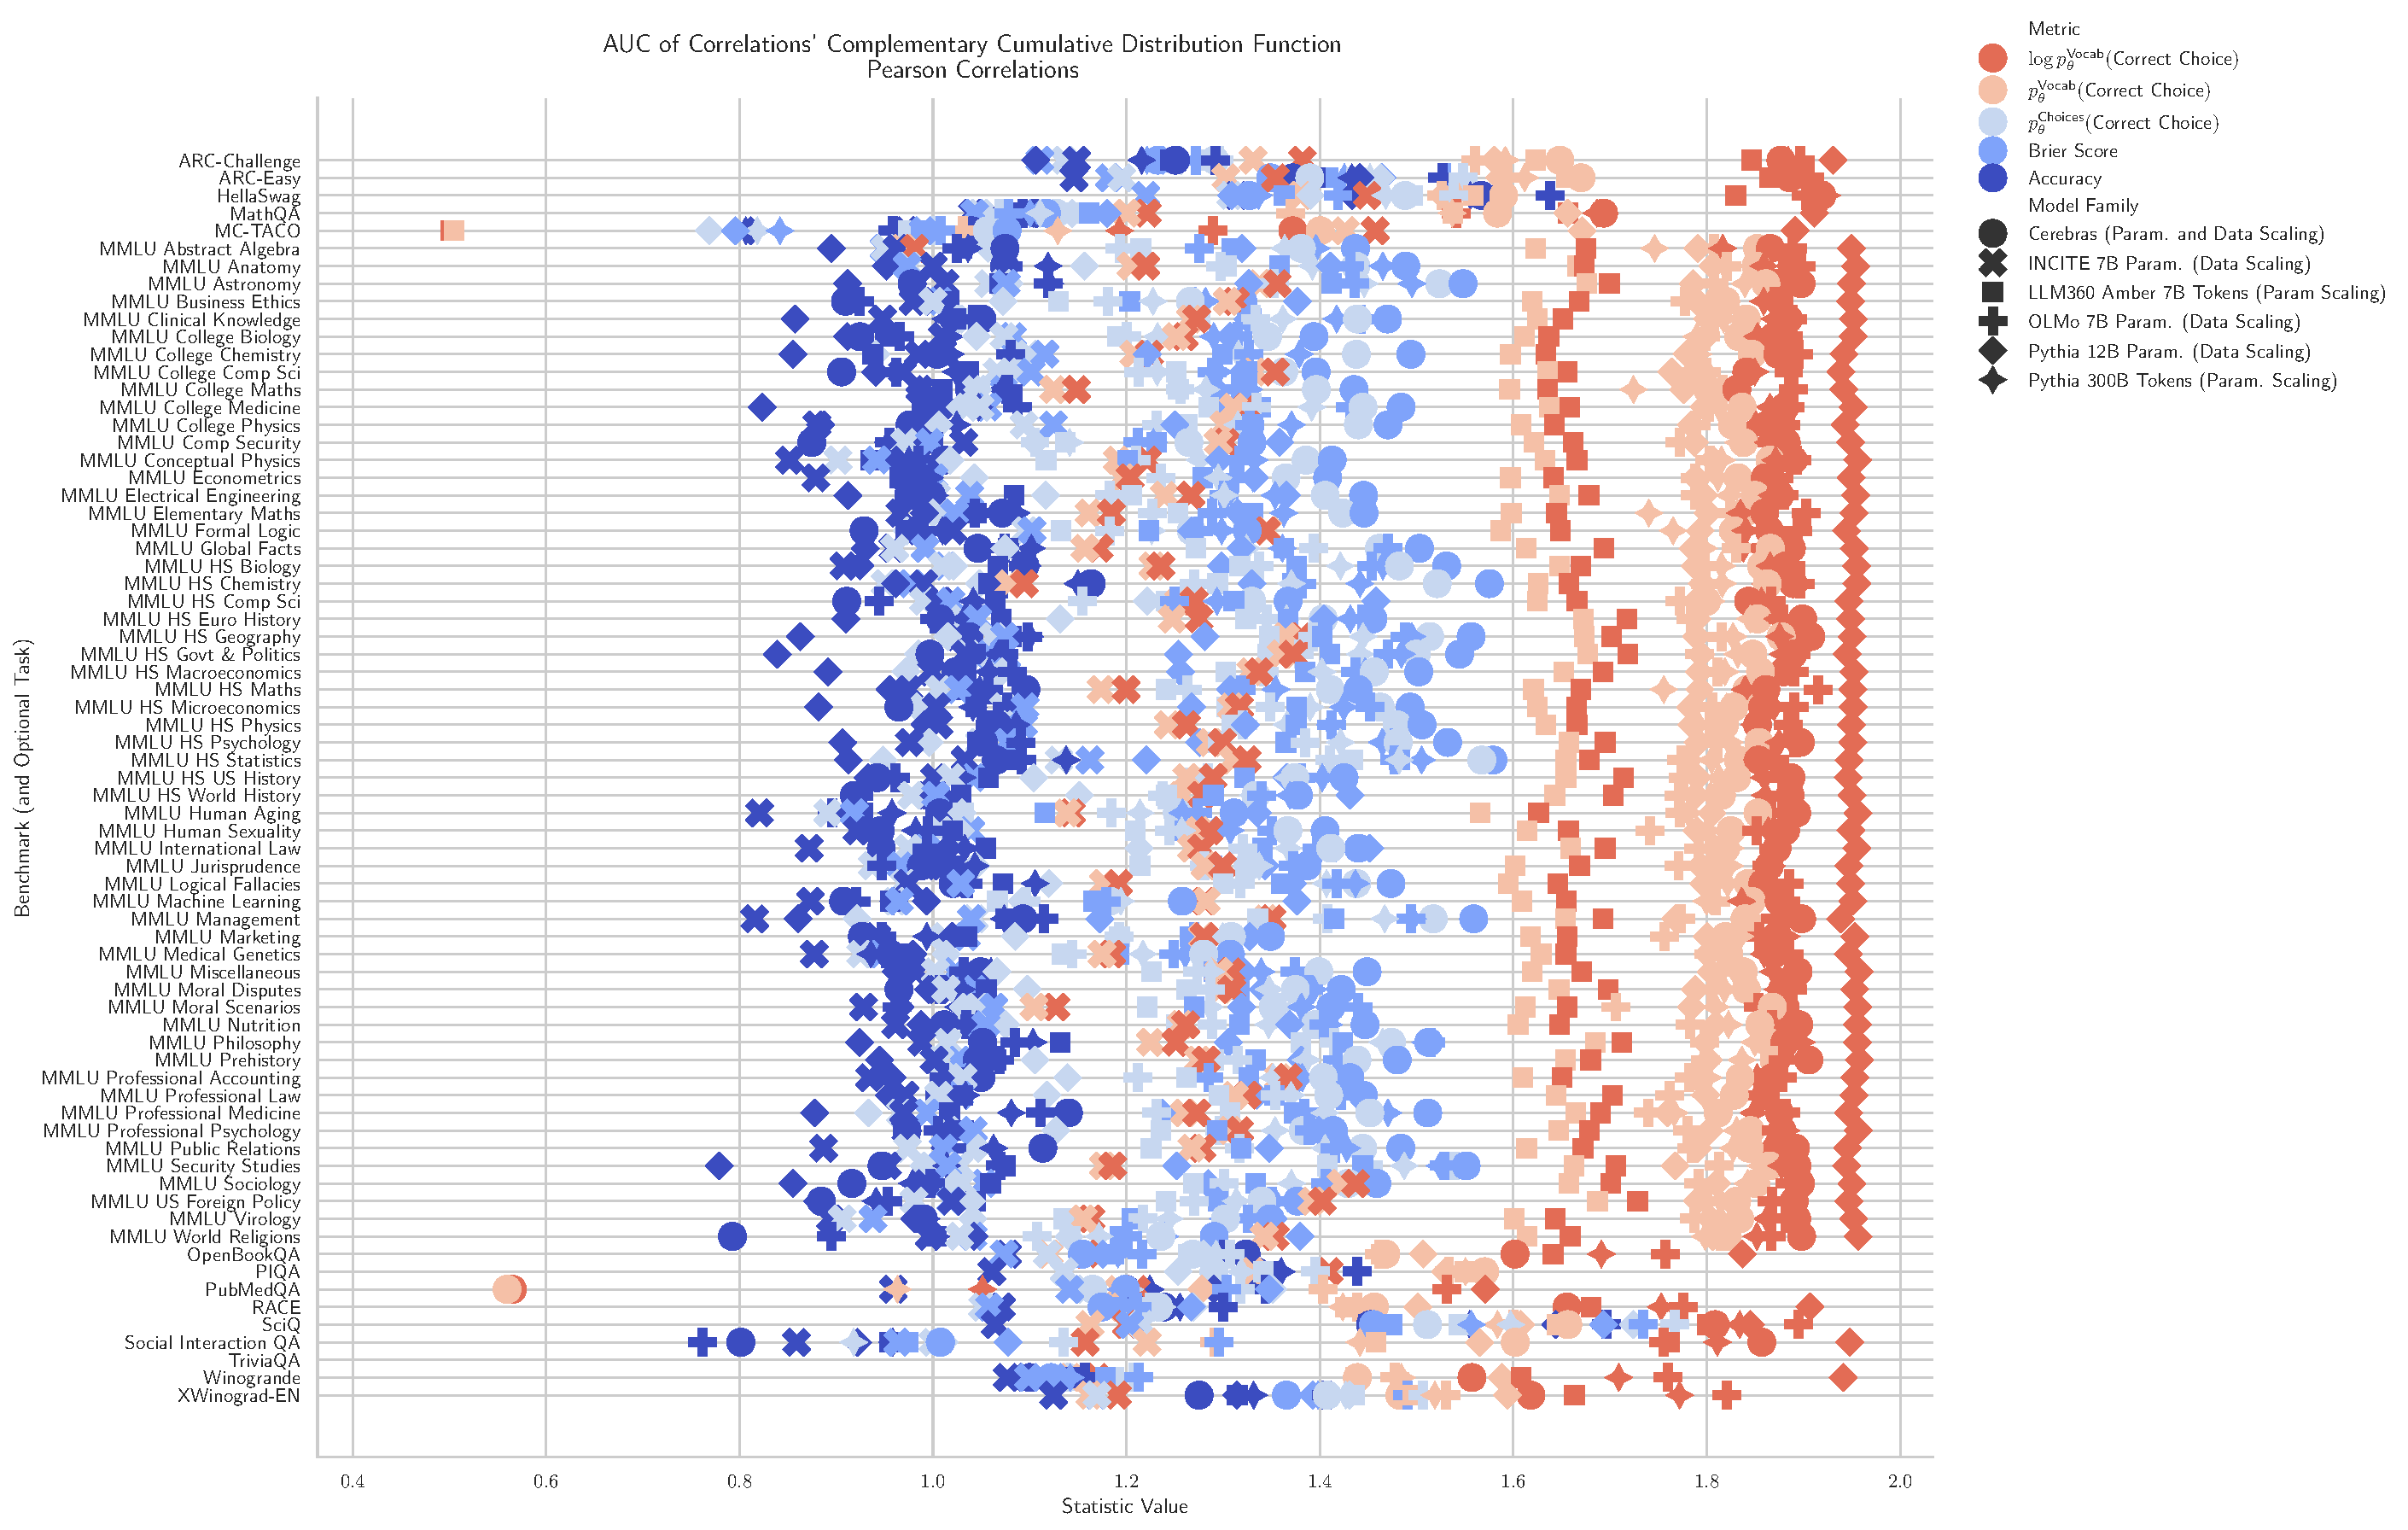
\includegraphics[width=0.9\textwidth]{figures/correlations_between_scores_and_compute/correlation_distribution_statistics/correlation_metric=pearson/benchmark_vs_pearson_correlation_distribution_statistic=statistics_correlation_auc_by_model_family_by_metric.pdf}
    \caption{\textbf{All four statistics of score-compute correlation distributions demonstrate that transforming $\log p_{\theta}^{\text{Vocab}}(\text{Correct Choice})$ into \texttt{Accuracy} causes score-compute correlations to deteriorate.} 
    We find a consistent trend that the sequence of transformations degrades score-compute correlations, as shown by the right-to-left \textbf{\textcolor{red}{$\log p_{\theta}^{\text{Vocab}}(\text{Correct Choice})$}}-to-\textbf{\textcolor{red!50!white}{$p_{\theta}^{\text{Vocab}}(\text{Correct Choice})$}}-to-\textbf{\textcolor{blue!50!white}{$p_{\theta}^{\text{Choices}}(\text{Correct Choice})$}}-or-\textbf{\textcolor{blue!75!white}{\texttt{Brier Score}}}-to-\textbf{\textcolor{blue!90!black}{\texttt{Accuracy}}} vertical stripes. This trend holds across benchmarks and model families for three correlation metrics (Spearman, Pearson and Kendall) and for four statistics of correlation distributions (mean, median, the area under the survival function, and negative Wasserstein distance from perfect correlation or perfect anti-correlation). See App. Figs. \ref{app:fig:compute_score_distribution_statistics_pearson}, \ref{app:fig:compute_score_distribution_statistics_spearman}, \ref{app:fig:compute_score_distribution_statistics_kendall} for other correlation metrics and other score-compute correlation distribution statistics.}
\label{fig:compute_score_distribution_statistics_spearman}
\end{figure*}


We demonstrate how the sequence of transformations affects the distribution of score-compute correlations using ARC Challenge \citep{clark2018arc} as an illustrative benchmark; we note that all other benchmarks exhibited similar patterns as well (App. \ref{app:sec:additional_score_compute_correlation_distributions}). We visualized the distributions via their complementary (empirical) cumulative distribution functions (complementary CDFs) (App. \ref{app:sec:survival_function}):
%
\begin{equation}
\hat{S}(c) \defeq \frac{1}{S} \sum_{s=1}^{S} \mathbbm{1}\{C_s > c\}
\label{eqn:empirical_survival_function},
\end{equation}
%
where $S$ is the number of samples in the benchmark and $C_s$ is the correlation (over the models in the model family) between compute and scores on the $s$-th sample in the benchmark. For a given threshold $c$, the complementary CDF $\hat{S}(c)$ returns the fraction of the benchmark's samples with score-compute correlations greater than the threshold $c$ (Fig. \ref{fig:compute_score_distribution_arc_challenge}A). Beginning with log likelihoods, approximately 90\% of samples exhibit score-compute correlations $> 0.75$, regardless of the model family (Fig. \ref{fig:compute_score_distribution_arc_challenge}A). Transforming negative log likelihoods into probability masses $p_{\theta}^{\text{Vocab}}(\text{Correct Choice})$ does not affect the distribution of score-compute correlations for Spearman and Kendall.
However, transforming $p_{\theta}^{\text{Vocab}}(\text{Correct Choice})$ into $p_{\theta}^{\text{Choices}}(\text{Correct Choice})$ decreases the distribution of score-compute correlations (Fig. \ref{fig:compute_score_distribution_arc_challenge}B), with only 40\% of samples having score-compute correlations $> 0.75$.
Transforming $p_{\theta}^{\text{Choices}}(\text{Correct Choice})$ into \texttt{Brier Score} has little-to-no effect (Fig. \ref{fig:compute_score_distribution_arc_challenge}C), but transforming into \texttt{Accuracy} (Fig. \ref{fig:compute_score_distribution_arc_challenge}D) furthers decreases score-compute correlations.
To quantitatively test whether these transformations indeed decrease the correlation between scores and compute, we measured four statistics of these score-compute correlation distributions: (1) the mean, (2) the median, (3) the area under the complementary CDF and (4) the negative\footnote{We chose the \textit{negative} Wasserstein distance for consistency with the other statistics: higher values correspond to higher correlations between scores and compute.} of the minimum of two Wasserstein distances: between the empirical correlation distribution and an ideal distribution of all correlations $=1$, and between the empirical distribution and an ideal distribution of all correlations $=-1$. Across the four summary statistics, for most benchmarks and for most model families, we discovered a consistent ordering of metrics of the score-compute correlation distributions (Fig. \ref{fig:compute_score_distribution_statistics_spearman}):
%
\begin{align*}
    &\text{Corr}\big(\text{Compute}, \textcolor{red}{\log p_{\theta}^{\text{Vocab}}(\text{Correct Choice})} \big) \\
    &\quad \geq \; \text{Corr}\big(\text{Compute}, \textcolor{red!50!white}{p_{\theta}^{\text{Vocab}}(\text{Correct Choice})}\big)\\
    &\quad  > \; \text{Corr}\big(\text{Compute}, \textcolor{blue!50!white}{p_{\theta}^{\text{Choices}}(\text{Correct Choice})}\big)\\
    &\quad \geq \; \text{Corr}\big(\text{Compute}, \textcolor{blue!75!white}{\texttt{Brier Score}}\big)\\
    &\quad  > \; \text{Corr}\big(\text{Compute}, \textcolor{blue!90!black}{\texttt{Accuracy}}\big)\\
\end{align*}
%
To quantitatively confirm that the correlation scores indeed follow this ordering, we computed what fraction of (benchmark, correlation metric, model family, correlation distribution statistic) tuples obey the ordering. To be maximally conservative, we checked for strict inequalities only. We found that across benchmarks, model families, and the 4 correlation distribution statistics, the claimed ordering of metrics held at least 82.4\% of the time for Pearson, 85.6\% for Spearman and 90.4\% for Kendall.

